\documentclass[11pt]{article}
\usepackage[utf8]{inputenc}  % gebruik de juiste 'character encoding'
\usepackage[dutch]{babel}    % definitie van de taal (Engels is de standaard)
\usepackage{hyperref}        % geef URLs netjes weer
\usepackage{booktabs}		 % mooiere tabellen
\usepackage{a4wide}          % papierformaat en marges
\usepackage{graphicx} 		 % Invoegen van plaatjes , ref: https://nl.sharelatex.com/learn/Inserting_Images
\usepackage{listings}
\usepackage{wrapfig}
\graphicspath{ {images/} }   % zet het pad voor de plaatjes
\pagestyle{plain}            % zet alleen paginanummering aan
% titel en auteur van het document
\title{Onderzoeks verslag DOOMotica}

\begin{document}
	\maketitle % maakt de title
	\begin{figure}[h]
		\centering
		
\includegraphics[width=\textwidth]{inholland}
	\end{figure}
	
	\newpage
	
	\tableofcontents
	\newpage
	\section{Domotica}
	De reden dat we dit project doen is zodat we de domotica in een huis zouden kunnen besturen. Hier voor maken we een webpagina waarop op onder andere de functies van Dahaus, spelletjes, tegeltjes voor je favoriete sites en nog wat andere tegeltjes voor je site geschiedenis.
	\newline
	\newline
	\newline
	\newline
	\section{Website bouwen}
	
	De opdracht voor de studenten is het maken van een website waar de gebruiker een account kan aanmaken en op dit account kan inloggen. Na het inloggen moet de gebruiker zijn favorieten site op de pagina kunnen zetten in de daar aangewezen tegels er voor. verder zijn er nog tegels voor de laatst bezochte sites. verder is er nog plek voor simpele spelletjes en als laatst moet de gebruiker Dahaus kunnen gebruiken.
	\newpage
	
	\section{Hindernissen}
	
	\subsection{geen database les}
	De leraar databases was in het begin van de periode afwezig. Hierdoor hebben we aan het begin van ons project niet goed met de database kunnen werken. Dit hebben we opgelost door zelf onderzoek te doen naar hoe SQL werkt en hoe je een database in elkaar zet. Later in de periode kwam de leraar weer op school en hebben we inhaal lessen gehad. Deze lessen hebben ons geholpen om ons database systeem te verbeteren en om onze comments die we naar de database sturen te verbeteren.
	
	\subsection{hashen}
	
	
	\newpage
	
	\section{Centrale vraag}
	In hoe verre zijn De studenten instaat tot het bouwen van een webpagina. Dit houd in een site met inlog systeem die ook gekoppeld is aan een database en werkende functie heeft zoals Dahaus en spelletjes om te spelen voor de gebruiker. Verder wil de opdrachtgever hoe uitgebreid de studenten de webpagina kunnen maken en wat de studenten nog meer verzinnen om als extra dingen er op te zetten. Denk hierbij bijvoorbeeld aan extra functie als een muziek speler. 
	
	\newpage
	
	\section{Deelvragen en onderzoeksvragen}
	\subsection{Dahaus}
	\subsection{spelltjes}
	De spelletjes die de studenten op de site moeten verwerken zijn simpele spelletjes voor de gebruiker om te spelen op de webpagina zelf. Er kunnen spelletjes op staan zoals: 
	\subsection{Tegeltjes}
	De Tegeltjes die op de site verwerkt zitten zijn voor de gebruiker. Om zelf in te vullen met zijn of haar eigen favorieten websites.
	\newpage
	
	\section{Verantwoording gebruikte methodes}
	\subsection{Create user}
	
	\subsection{Inloggen}
	Voor het inlog gedeelte van het systeem zijn de studenten zelf gaan programmeren. Dit omdat de studenten dit een leuke uitdaging leek. Bij het maken van de inlog hebben de studenten een psd gemaakt zoals te zien is in Figuur \ref{Login}. Het Programma is opgebouwd uit een aantal delen deze zijn Het ophalen van het wachtwoord uit de Database. Vervolgens het wachtwoord omzetten naar byte, daarna dan het opsplitsen van de Salt en de Hash. vervolgens de Slat voor het ingevulde wachtwoord zetten. Dit Wordt dan gehashed en als laatst word er vergeleken of de hash van het wachtwoord uit de database en het net gehashde wachtwoord het zelfde zijn, als dit zo is dan word er een cookie gemaakt die de gebruikersnaam onthoud en de gebruiker door stuurt naar de homepage. Wanneer dit niet het geval is krijgt de gebruiker een foutmelding dat het wachtwoord niet correct is. De code is te zien in Figuur \ref{LoginCode}.
	\newpage
	
	\section{Analyse van de gegevens}
	
	\subsection{Dataverzameling}
	De Studenten hebben voor een groot deel gebruik gemaakt van de gegeven powerpoints van de lessen Webprogrammeren. ook hebben we een aantal dingen opgezocht op internet hier de links die we gebruikt hebben: \url{https://msdn.microsoft.com/en-us/library/ms525800(v=vs.90).aspx} (bekeken op \date{19-01-2018}, Geschreven door Microsoft), \newline \url{https://stackoverflow.com/questions/13058574/check-if-cookie-exists}(Bekeken op \date{19-01-2018}, geschreven door zmbq).
	
	\subsection{Analyse}
	De powerpoints waren van een betrouwbare bron. Ze komen namelijk van hun docent die ze les heeft gegeven in webprogrameren en het is ook 1 van de docenten die het project beoordeeld hierdoor weten de studenten ook meteen dat het op de manier gaat als de opdrachtgever wil. De eerste link is afkomstig van Microsoft een betrouwbare bron, omdat het programma waar de studenten hun webpagina op maken ook van Microsoft is. De Tweede links is van de site stackoverflow op deze site stellen mensen vragen over dingen waar ze niet uitkomen met hun programma's. De antwoorden zijn niet altijd betrouwbaar, maar in dit geval werkte het antwoord wel.

	\subsection{Deelconclusie/ aanbeveling}
	De studenten zijn er achtergekomen dat de powerpoints heel handig zijn om bij de hand te hebben voor als je ergens niet op komt. Verder zijn de voorbeelden van Microsoft handig om op te zoeken als je iets niet meer compleet weet. De site stackoverflow is handig als je weet wat je wilt alleen niet weet hoe je het uitvoerd. De studenten zouden aanbevelen om zeker de powerpoints te gebruiken en als je het daar niet in kunt vinden kun je altijd nog internet raadplegen. 
	\newpage
	
	\section{Eindconclusie}
	De studenten zijn er achter gekomen dat het meer werk is dan alleen maar een paar dingen op de pagina slepen zoals in de lessen werd gedaan om, maar dat er veel meer bij komt kijken bij een echte webpagina maken met alle eisen zoals beschreven staat in Hoofdstuk 2 staat beschreven. Verder is het handig als zoals bij de studenten gebeurde dat er een les als database uitvalt voor het begin van de periode dat je er zelf gewoon mee aan de slag gaat dan word je achterstand niet te groot.
	
	
	\section{Aanbeveling}
	De aanbeveling van de studenten is om het werk niet te onderschatten en op tijd er mee te beginnen zodat je tijd over kan houden voor extra dingen. Die je op je webpagina wilt zetten. Verder als er een les niet gegeven word om de één of andere reden zoek iemand die er het begrijpt en kan uitleggen en vraag om hulp wanneer nodig, ook aan je groepsgenoten. het is beter hulp te vragen dan het slecht product te leveren.  
	
	\newpage
	
	\section{bijlagen}
	
	\begin{figure}[h]
		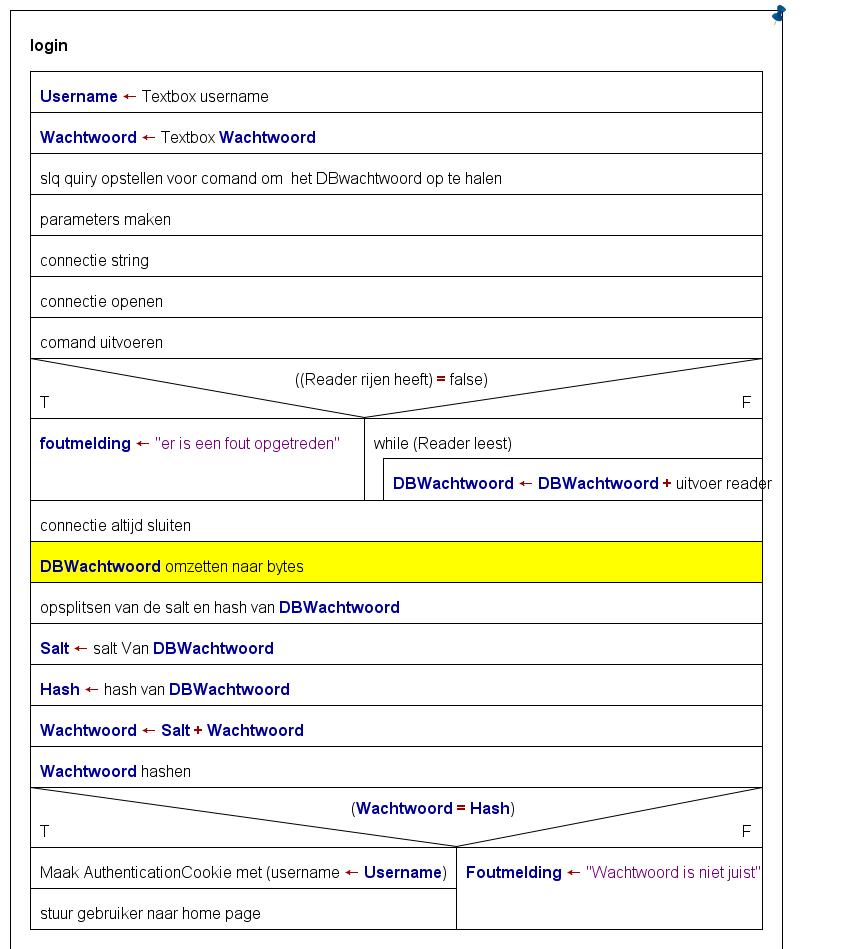
\includegraphics[scale=0.4]{Login}
		\caption{psd van de Login}
		\label{Login}
	\end{figure}
	\newpage
	\begin{figure}[h]
		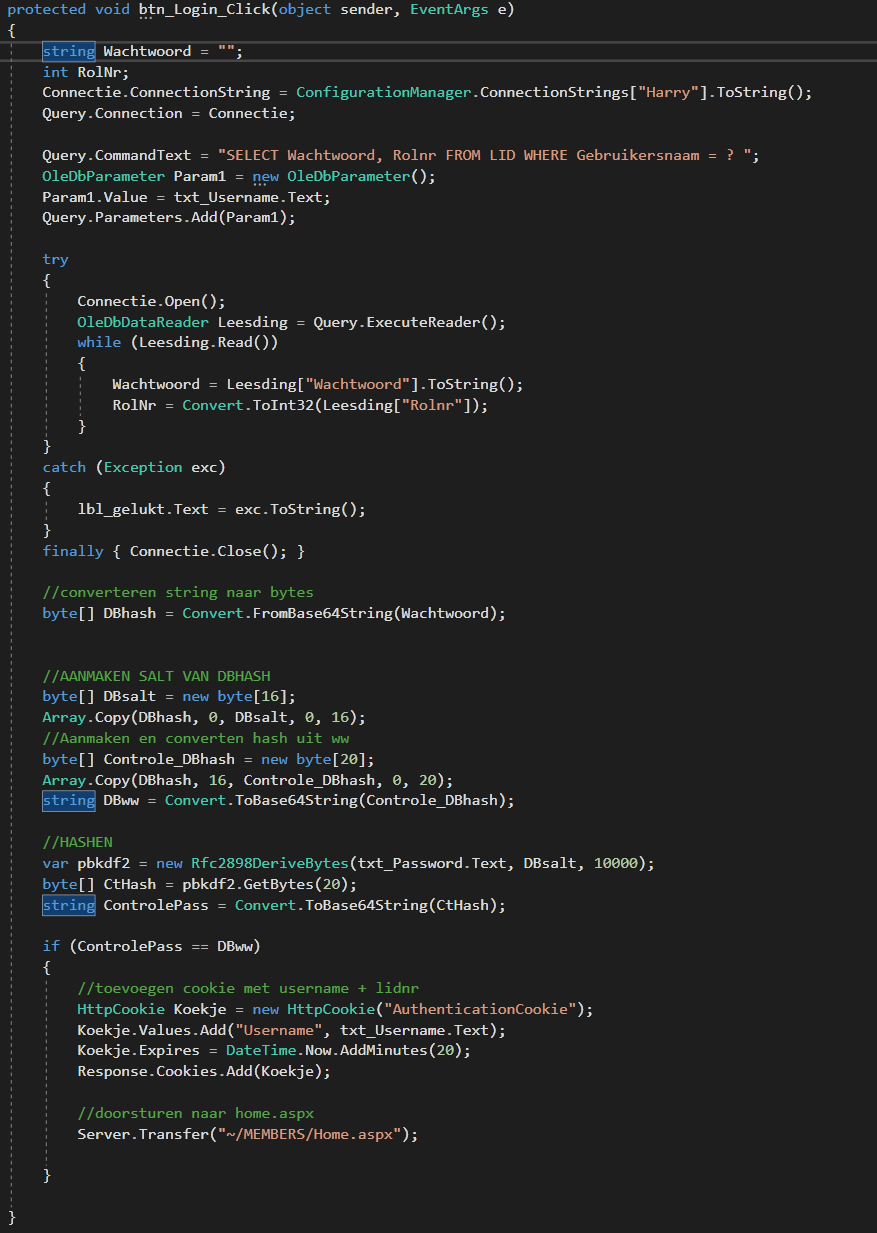
\includegraphics[scale=0.8]{CodeLogin}
		\caption{Code van de login}
		\label{LoginCode}
	\end{figure}
	\newpage
	
\end{document}